\chapter{Diagrammes et schémas techniques}

Cette annexe présente les diagrammes techniques détaillés qui complètent l'analyse et la conception de la plateforme municipale d'Azrou.

\section{Diagrammes d'architecture}

\subsection{Architecture globale du système}

\begin{figure}[H]
\centering
\begin{tikzpicture}[
    node distance=2cm,
    box/.style={rectangle, draw, fill=blue!20, minimum width=3cm, minimum height=1cm, text centered},
    database/.style={cylinder, draw, fill=green!20, minimum width=2cm, minimum height=1.5cm, text centered},
    cloud/.style={ellipse, draw, fill=yellow!20, minimum width=2cm, minimum height=1cm, text centered}
]

% Couche présentation
\node[box] (frontend) {Frontend React.js};

% Couche API
\node[box, below=of frontend] (api) {API REST Express.js};

% Couche métier
\node[box, below left=of api] (auth) {Authentification JWT};
\node[box, below right=of api] (business) {Logique Métier};

% Couche données
\node[database, below=of auth] (mongodb) {MongoDB Atlas};
\node[cloud, below=of business] (cloudinary) {Cloudinary};

% Services externes
\node[cloud, right=of cloudinary] (email) {Service Email};
\node[cloud, right=of email] (sms) {Service SMS};

% Connexions
\draw[->] (frontend) -- (api) node[midway, right] {HTTPS/REST};
\draw[->] (api) -- (auth);
\draw[->] (api) -- (business);
\draw[->] (auth) -- (mongodb) node[midway, left] {Requêtes};
\draw[->] (business) -- (mongodb);
\draw[->] (business) -- (cloudinary) node[midway, above] {Upload};
\draw[->] (business) -- (email);
\draw[->] (business) -- (sms);

\end{tikzpicture}
\caption{Architecture globale de la plateforme municipale}
\label{fig:architecture-globale}
\end{figure}

\subsection{Architecture de sécurité}

\begin{figure}[H]
\centering
\begin{tikzpicture}[
    node distance=2cm,
    secure/.style={rectangle, draw=red!50, fill=red!10, thick, minimum width=2.5cm, minimum height=1cm},
    normal/.style={rectangle, draw=blue!50, fill=blue!10, minimum width=2.5cm, minimum height=1cm}
]

\node[normal] (client) {Client Web};
\node[secure, below=of client] (https) {HTTPS/TLS};
\node[secure, below=of https] (cors) {CORS Policy};
\node[secure, below=of cors] (auth) {JWT Auth};
\node[secure, below=of auth] (rbac) {RBAC};
\node[normal, below=of rbac] (api) {API Endpoints};
\node[secure, below=of api] (validation) {Validation};
\node[secure, below=of validation] (sanitization) {Sanitisation};
\node[normal, below=of sanitization] (database) {Base de données};

% Flèches de sécurité
\draw[->, red, thick] (client) -- (https) node[midway, right] {Chiffrement};
\draw[->, red, thick] (https) -- (cors) node[midway, right] {Origin Control};
\draw[->, red, thick] (cors) -- (auth) node[midway, right] {Token Check};
\draw[->, red, thick] (auth) -- (rbac) node[midway, right] {Role Check};
\draw[->, blue] (rbac) -- (api);
\draw[->, red, thick] (api) -- (validation) node[midway, right] {Input Valid};
\draw[->, red, thick] (validation) -- (sanitization) node[midway, right] {Data Clean};
\draw[->, blue] (sanitization) -- (database);

\end{tikzpicture}
\caption{Couches de sécurité de l'application}
\label{fig:securite}
\end{figure}

\section{Diagrammes de flux de données}

\subsection{Flux d'authentification utilisateur}

\begin{figure}[H]
\centering
\begin{tikzpicture}[
    node distance=1.5cm,
    process/.style={rectangle, draw, fill=blue!20, minimum width=2cm, minimum height=0.8cm},
    decision/.style={diamond, draw, fill=yellow!20, minimum width=1.5cm, minimum height=1cm},
    data/.style={parallelogram, draw, fill=green!20, minimum width=2cm, minimum height=0.8cm}
]

\node[process] (start) {Début};
\node[data, below=of start] (input) {Email + Password};
\node[process, below=of input] (validate) {Validation};
\node[decision, below=of validate] (valid) {Valide?};
\node[process, below left=of valid] (error) {Erreur};
\node[process, below=of valid] (check) {Vérifier DB};
\node[decision, below=of check] (exists) {Utilisateur existe?};
\node[process, left=of exists] (notfound) {Non trouvé};
\node[process, below=of exists] (compare) {Comparer MDP};
\node[decision, below=of compare] (match) {Match?};
\node[process, left=of match] (wrongpwd) {MDP incorrect};
\node[process, below=of match] (token) {Générer JWT};
\node[data, below=of token] (response) {Token + User};
\node[process, below=of response] (end) {Fin};

% Connexions
\draw[->] (start) -- (input);
\draw[->] (input) -- (validate);
\draw[->] (validate) -- (valid);
\draw[->] (valid) -- node[left] {Non} (error);
\draw[->] (valid) -- node[right] {Oui} (check);
\draw[->] (check) -- (exists);
\draw[->] (exists) -- node[above] {Non} (notfound);
\draw[->] (exists) -- node[right] {Oui} (compare);
\draw[->] (compare) -- (match);
\draw[->] (match) -- node[above] {Non} (wrongpwd);
\draw[->] (match) -- node[right] {Oui} (token);
\draw[->] (token) -- (response);
\draw[->] (response) -- (end);

% Retours d'erreur
\draw[->] (error) -- ++(-2,0) |- (end);
\draw[->] (notfound) -- ++(-1,0) |- (end);
\draw[->] (wrongpwd) -- ++(-1,0) |- (end);

\end{tikzpicture}
\caption{Flux d'authentification utilisateur}
\label{fig:auth-flow}
\end{figure}

\subsection{Flux de prise de rendez-vous}

\begin{figure}[H]
\centering
\begin{tikzpicture}[
    node distance=1.2cm,
    process/.style={rectangle, draw, fill=blue!20, minimum width=2.5cm, minimum height=0.8cm},
    decision/.style={diamond, draw, fill=yellow!20, minimum width=2cm, minimum height=1cm},
    data/.style={parallelogram, draw, fill=green!20, minimum width=2cm, minimum height=0.8cm}
]

\node[process] (start) {Sélection service};
\node[process, below=of start] (calendar) {Afficher calendrier};
\node[process, below=of calendar] (select) {Sélectionner créneau};
\node[decision, below=of select] (available) {Disponible?};
\node[process, right=of available] (unavailable) {Afficher erreur};
\node[process, below=of available] (form) {Formulaire détails};
\node[process, below=of form] (validate) {Validation données};
\node[decision, below=of validate] (valid) {Données valides?};
\node[process, right=of valid] (error) {Afficher erreurs};
\node[process, below=of valid] (save) {Enregistrer RDV};
\node[process, below=of save] (notify) {Notification};
\node[data, below=of notify] (confirmation) {Confirmation};
\node[process, below=of confirmation] (end) {Fin};

% Connexions principales
\draw[->] (start) -- (calendar);
\draw[->] (calendar) -- (select);
\draw[->] (select) -- (available);
\draw[->] (available) -- node[above] {Non} (unavailable);
\draw[->] (available) -- node[right] {Oui} (form);
\draw[->] (form) -- (validate);
\draw[->] (validate) -- (valid);
\draw[->] (valid) -- node[above] {Non} (error);
\draw[->] (valid) -- node[right] {Oui} (save);
\draw[->] (save) -- (notify);
\draw[->] (notify) -- (confirmation);
\draw[->] (confirmation) -- (end);

% Retours
\draw[->] (unavailable) -- ++(0,1) -| (calendar);
\draw[->] (error) -- ++(0,1) -| (form);

\end{tikzpicture}
\caption{Processus de prise de rendez-vous}
\label{fig:appointment-flow}
\end{figure}

\section{Modèle de données détaillé}

\subsection{Diagramme Entité-Relation}

\begin{figure}[H]
\centering
\begin{tikzpicture}[
    entity/.style={rectangle, draw, fill=blue!20, minimum width=3cm, minimum height=2cm},
    attribute/.style={ellipse, draw, fill=green!20, minimum width=1.5cm, minimum height=0.8cm},
    relationship/.style={diamond, draw, fill=yellow!20, minimum width=2cm, minimum height=1cm}
]

% Entités principales
\node[entity] (user) at (0,0) {\textbf{UTILISATEUR}\\id, nom, email\\phone, role, statut};
\node[entity] (appointment) at (6,0) {\textbf{RENDEZ-VOUS}\\id, date, heure\\statut, notes};
\node[entity] (service) at (3,4) {\textbf{SERVICE}\\id, nom, description\\durée, prix};
\node[entity] (department) at (3,-4) {\textbf{DÉPARTEMENT}\\id, nom, description\\responsable};

% Relations
\node[relationship] (prend) at (3,0) {PREND};
\node[relationship] (propose) at (3,2) {PROPOSE};
\node[relationship] (gere) at (3,-2) {GÈRE};

% Connexions
\draw (user) -- (prend);
\draw (prend) -- (appointment);
\draw (service) -- (propose);
\draw (propose) -- (appointment);
\draw (department) -- (gere);
\draw (gere) -- (service);

% Cardinalités
\node at (1.5,0.3) {1,n};
\node at (4.5,0.3) {1,1};
\node at (3,1.3) {1,n};
\node at (3,2.7) {1,1};
\node at (3,-1.3) {1,1};
\node at (3,-2.7) {1,n};

\end{tikzpicture}
\caption{Modèle Entité-Relation simplifié}
\label{fig:er-model}
\end{figure}

\subsection{Structure de la base de données MongoDB}

\begin{figure}[H]
\centering
\lstset{
    basicstyle=\tiny\ttfamily,
    frame=single,
    breaklines=true,
    captionpos=b
}
\begin{lstlisting}[language=json, caption=Structure JSON des collections MongoDB]
// Collection: users
{
  "_id": ObjectId,
  "name": String,
  "email": String (unique, indexed),
  "password": String (hashed),
  "phone": String,
  "role": String (enum),
  "isActive": Boolean,
  "createdAt": ISODate,
  "preferences": {
    "language": String,
    "notifications": Object
  }
}

// Collection: appointments  
{
  "_id": ObjectId,
  "userId": ObjectId (ref: users),
  "serviceId": ObjectId (ref: services),
  "date": ISODate,
  "time": String,
  "status": String (enum),
  "notes": String,
  "createdAt": ISODate,
  "metadata": {
    "source": String,
    "priority": Number
  }
}

// Collection: services
{
  "_id": ObjectId,
  "name": String,
  "description": String,
  "departmentId": ObjectId (ref: departments),
  "duration": Number (minutes),
  "price": Number,
  "isActive": Boolean,
  "requirements": [String],
  "schedule": {
    "days": [Number],
    "hours": {
      "start": String,
      "end": String
    }
  }
}
\end{lstlisting}
\end{figure}

\section{Diagrammes de déploiement}

\subsection{Infrastructure cloud}

\begin{figure}[H]
\centering
\begin{tikzpicture}[
    cloud/.style={ellipse, draw, fill=blue!20, minimum width=3cm, minimum height=1.5cm},
    server/.style={rectangle, draw, fill=green!20, minimum width=2.5cm, minimum height=1cm},
    database/.style={cylinder, draw, fill=yellow!20, minimum width=2cm, minimum height=1.2cm}
]

% Cloud providers
\node[cloud] (vercel) at (0,4) {Vercel\\Frontend};
\node[cloud] (render) at (6,4) {Render\\Backend};
\node[cloud] (atlas) at (3,1) {MongoDB Atlas\\Database};

% Services
\node[server] (frontend) at (0,2) {React App\\Build};
\node[server] (backend) at (6,2) {Node.js API\\Express};
\node[database] (db) at (3,-1) {Collections\\& Indexes};

% CDN et services
\node[cloud] (cloudinary) at (-3,1) {Cloudinary\\Media};
\node[cloud] (email) at (9,1) {SendGrid\\Email};

% Connexions
\draw[->] (vercel) -- (frontend);
\draw[->] (render) -- (backend);
\draw[->] (atlas) -- (db);
\draw[->] (frontend) -- (backend) node[midway, above] {HTTPS API};
\draw[->] (backend) -- (db) node[midway, right] {Mongoose ODM};
\draw[->] (backend) -- (cloudinary) node[midway, above] {Upload API};
\draw[->] (backend) -- (email) node[midway, above] {SMTP};

\end{tikzpicture}
\caption{Architecture de déploiement cloud}
\label{fig:deployment}
\end{figure}

\subsection{Flux de données en production}

\begin{figure}[H]
\centering
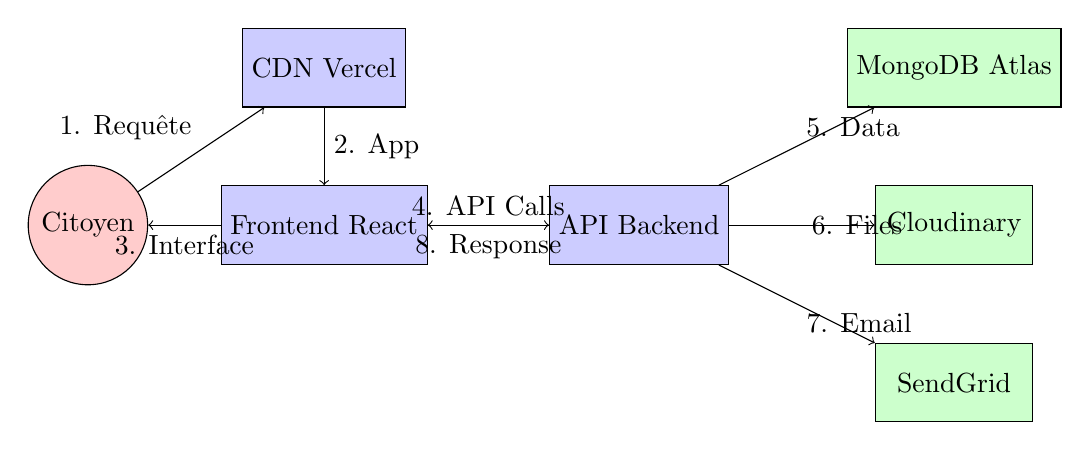
\begin{tikzpicture}[
    user/.style={circle, draw, fill=red!20, minimum size=1cm},
    service/.style={rectangle, draw, fill=blue!20, minimum width=2cm, minimum height=1cm},
    external/.style={rectangle, draw, fill=green!20, minimum width=2cm, minimum height=1cm}
]

\node[user] (citizen) at (0,0) {Citoyen};
\node[service] (cdn) at (3,2) {CDN Vercel};
\node[service] (frontend) at (3,0) {Frontend React};
\node[service] (api) at (7,0) {API Backend};
\node[external] (mongodb) at (11,2) {MongoDB Atlas};
\node[external] (cloudinary) at (11,0) {Cloudinary};
\node[external] (sendgrid) at (11,-2) {SendGrid};

% Flux de données
\draw[->] (citizen) -- (cdn) node[midway, above left] {1. Requête};
\draw[->] (cdn) -- (frontend) node[midway, right] {2. App};
\draw[->] (frontend) -- (citizen) node[midway, below] {3. Interface};
\draw[->] (frontend) -- (api) node[midway, above] {4. API Calls};
\draw[->] (api) -- (mongodb) node[midway, above right] {5. Data};
\draw[->] (api) -- (cloudinary) node[midway, right] {6. Files};
\draw[->] (api) -- (sendgrid) node[midway, below right] {7. Email};
\draw[->] (api) -- (frontend) node[midway, below] {8. Response};

\end{tikzpicture}
\caption{Flux de données en production}
\label{fig:data-flow-prod}
\end{figure}

Cette annexe complète la documentation technique avec les diagrammes essentiels pour comprendre l'architecture, les flux de données et le déploiement de la plateforme municipale d'Azrou.
